\chapter{A recurrence for rational approximants}
\label{cb_ch_recurrence}

The elementary series gives rational approximations to $G$ term by term.
Zudilin's recurrence gives a different family whose errors decrease much
faster \cite{Zudilin2003}. Its coefficients and initial values are rational,
so every finite calculation can be performed exactly. The recurrence is
also a useful structural object: a two dimensional transfer matrix carries
each pair of adjacent values to the next, and a determinant tracks the
independence of its two distinguished solutions.

We first define the sequences as rational algebraic objects. We then state
the external theorem identifying their limit with Catalan's constant and
their exponential rates. This separates what follows from the recurrence
alone from what requires its analytic interpretation.

\section{The equation and its initial data}

For integer $n\geq0$, set
\begin{align}
 p(n)&=20n^2-8n+1,\label{cb_eq_p_polynomial}\\
 q(n)&=3520n^6+5632n^5+2064n^4-384n^3-156n^2+16n+7.
 \label{cb_eq_q_polynomial}
\end{align}
For $n\geq1$, abbreviate the leading and trailing coefficients by
\begin{equation}\label{cb_eq_a_c_def}
 a_n=(2n+1)^2(2n+2)^2p(n),\qquad
 c_n=(2n-1)^2(2n)^2p(n+1).
\end{equation}
The recurrence is
\begin{equation}\label{cb_eq_zudilin_recurrence}
 a_nw_{n+1}-q(n)w_n-c_nw_{n-1}=0,\qquad n\geq1.
\end{equation}
The signs of the last two terms are part of the normalization. Solving
forward gives $w_{n+1}=(q(n)w_n+c_nw_{n-1})/a_n$.

\begin{definition}[The distinguished rational sequences]\label{cb_def_uv}
Let $(u_n)_{n\geq0}$ and $(v_n)_{n\geq0}$ satisfy
\eqref{cb_eq_zudilin_recurrence}, with
\begin{equation}\label{cb_eq_uv_initial}
 (u_0,u_1)=\left(1,\frac74\right),\qquad
 (v_0,v_1)=\left(0,\frac{13}{8}\right).
\end{equation}
Their rational approximants are
\begin{equation}\label{cb_eq_r_def}
 r_n=\frac{v_n}{u_n}.
\end{equation}
\end{definition}

The notation $a_n,c_n$ in this chapter and the next denotes recurrence
coefficients. The later source notation $a_n,b_n$ is translated explicitly
when it occurs, and the cleared packet coefficients $A_{n,m},B_{n,m}$ have
two indices. These are different objects.

The forward equation starts at $n=1$. Substituting $n=0$ into its polynomial
expression would remove the trailing term and impose $4w_1=7w_0$. Although
the initial values of $u$ happen to satisfy that extra equation, those of
$v$ do not. It is therefore not a valid additional recurrence condition
for the pair. At $n=1$, both $w_0$ and $w_1$ are already specified and
$w_2$ is the first value to be computed.

\section{Existence, uniqueness and positivity}

\begin{proposition}[Well defined rational solutions]\label{cb_prop_forward}
Every initial pair $(w_0,w_1)\in\Q^2$ determines exactly one rational
sequence satisfying \eqref{cb_eq_zudilin_recurrence}. In particular the
sequences in Definition~\ref{cb_def_uv} exist uniquely. Moreover,
\[
 u_n>0\quad(n\geq0),\qquad v_n>0\quad(n\geq1),\qquad v_0=0.
\]
\end{proposition}

\begin{proof}
Completing the square gives
\[
 p(n)=20\left(n-\frac15\right)^2+\frac15>0.
\]
Thus $a_n,c_n>0$ for $n\geq1$. Also, for such $n$,
\[
 2064n^4-384n^3-156n^2\geq1524n^4>0,
\]
because $n^3\leq n^4$ and $n^2\leq n^4$. All the remaining terms of $q(n)$
are positive, so $q(n)>0$. Division by $a_n$ therefore makes forward
iteration possible. It preserves rationality and determines the next term
uniquely. Induction proves existence and uniqueness at every index.

The initial $u$ values are positive, and each subsequent value is a positive
linear combination of its two predecessors. For $v$, the initial $v_0$ is
zero and $v_1>0$. The first forward step gives $v_2>0$, and the same
induction applies thereafter. Consequently the quotient $r_n$ is defined
at every index.
\end{proof}

These conclusions concern an infinite sequence but require only the
recurrence and a finite induction rule. They do not require a numerical
run through a large terminal index. The computer checks test whether an
implementation follows the rule correctly.

The solution space also has a concrete basis. For any rational solution
$w$, put
\[
 x=w_0,\qquad y=\frac8{13}\left(w_1-\frac74w_0\right).
\]
The sequence $xu_n+yv_n$ has the same initial pair as $w_n$. By uniqueness,
\begin{equation}\label{cb_eq_solution_basis}
 w_n=xu_n+yv_n\qquad(n\geq0).
\end{equation}
Thus the entire space of rational solutions is two dimensional. The factor
$13/8$ in the initial data is nonzero, so there is no degeneracy in this
basis calculation. The same argument works for real initial values,
yielding the two dimensional real solution space.

\begin{figure}[tbp]
\centering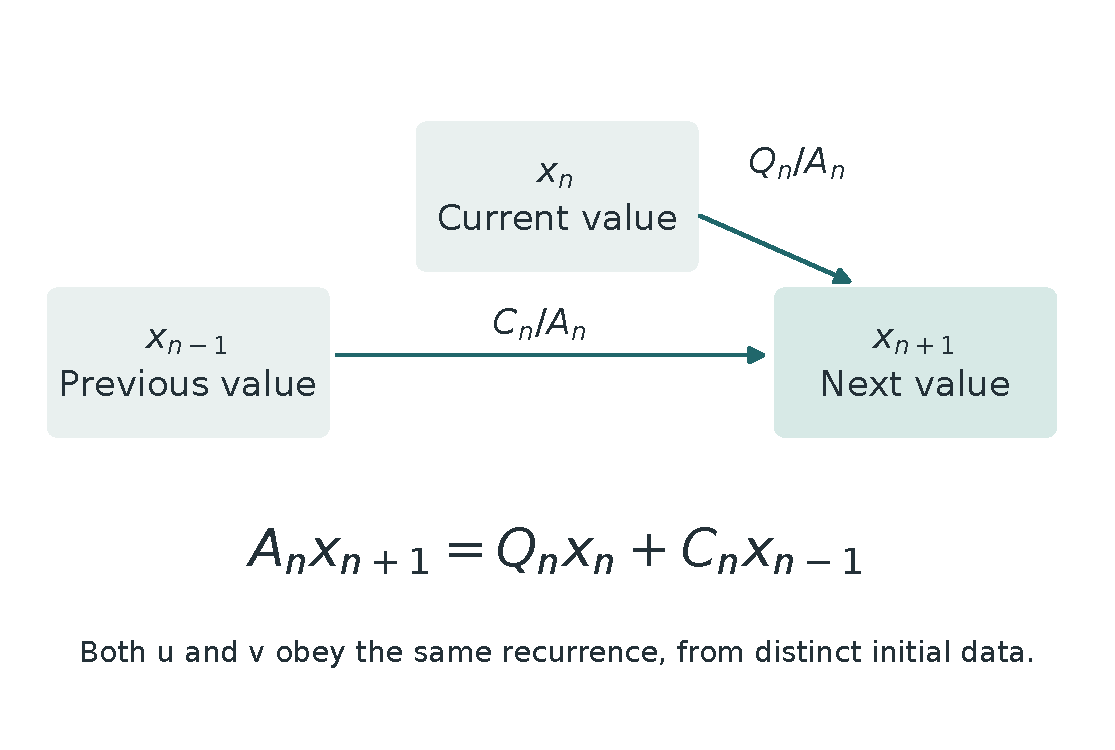
\includegraphics[width=0.93\linewidth]{../visual/figures/09_recurrence_structure.pdf}
\caption{Two preceding values determine the next rational value. The
forward rule begins at $n=1$ and uses the stated initial pair. Here and in
subsequent recurrence diagrams, $A_n=a_n$, $Q_n=q(n)$ and $C_n=c_n$.}
\label{cb_fig_recurrence}
\end{figure}

\section{Two complete forward steps}

The first steps expose all constants and signs. At $n=1$,
\[
 p(1)=13,\quad p(2)=65,\quad q(1)=10699,\qquad
 a_1=1872,\quad c_1=260.
\]
For $u$, the recurrence gives
\[
 u_2=\frac{10699(7/4)+260}{1872}
     =\frac{75933/4}{1872}=\frac{649}{64}.
\]
For $v$, its zero initial term removes the trailing contribution:
\[
 v_2=\frac{10699(13/8)+260\cdot0}{1872}
     =\frac{139087/8}{1872}=\frac{10699}{1152}.
\]
Therefore the second rational approximant is
\[
 r_2=\frac{10699}{11682}.
\]

At $n=2$ the coefficients become
\[
 p(2)=65,\quad p(3)=157,\quad q(2)=434871,\qquad
 a_2=58500,\quad c_2=22608.
\]
Using the fractions just obtained,
\begin{align*}
 u_3
 &=\frac{434871(649/64)+22608(7/4)}{58500}\\
 &=\frac{284763375/64}{58500}=\frac{19471}{256},\\[3pt]
 v_3
 &=\frac{434871(10699/1152)+22608(13/8)}{58500}\\
 &=\frac{521667445/128}{58500}=\frac{8025653}{115200}.
\end{align*}
It follows that $r_3=8025653/8761950$. All these values were also checked
against the recovered exact rational script. A floating point calculation
is unnecessary for the equality at any stage.

The first ratios are $r_0=0$ and $r_1=13/14$. The subsequent values lie
near the decimal for $G$, but proximity is only a first observation.
Chapter~\ref{cb_ch_wronskian} proves exact nested brackets and an error
sign at every index. The external identification below then makes those
brackets enclosures of Catalan's constant itself.

\section{The transfer matrix and its determinant}

Normalize the recurrence by putting
\[
 \alpha_n=\frac{q(n)}{a_n},\qquad
 \beta_n=\frac{c_n}{a_n}\qquad(n\geq1).
\]
Both quantities are positive rationals. For the adjacent state vector
$X_n(w)=(w_n,w_{n-1})^{\mathsf T}$, define
\begin{equation}\label{cb_eq_transfer}
 M_n=\begin{pmatrix}\alpha_n&\beta_n\\1&0\end{pmatrix}.
 \qquad X_{n+1}(w)=M_nX_n(w).
\end{equation}
Hence
\[
 X_{N+1}(w)=M_NM_{N-1}\cdots M_1X_1(w)\qquad(N\geq1).
\]
The order of multiplication follows the temporal order: $M_1$ acts first.
This is a product of changing matrices, not a power of one fixed matrix.

The determinant is
\[
 \det M_n=-\beta_n=-\frac{c_n}{a_n}<0.
\]
Every transfer is invertible, with
\[
 M_n^{-1}=\begin{pmatrix}0&1\\1/\beta_n&-\alpha_n/\beta_n\end{pmatrix}.
\]
An adjacent pair at index $n+1$ therefore determines the preceding pair at
index $n$, within the stated recurrence domain. This does not extend the
equation through $n=0$, where the trailing coefficient would vanish.

The two distinguished solutions can be collected into the fundamental
matrix
\[
 \mathcal F_n=
 \begin{pmatrix}u_n&v_n\\u_{n-1}&v_{n-1}\end{pmatrix},\qquad n\geq1.
\]
It satisfies $\mathcal F_{n+1}=M_n\mathcal F_n$. Its initial determinant is
\[
 \det\mathcal F_1=
 \det\begin{pmatrix}7/4&13/8\\1&0\end{pmatrix}=-\frac{13}{8}.
\]
Multiplicativity of determinants now gives
\[
 \det\mathcal F_{N+1}
 =-\frac{13}{8}\prod_{n=1}^N(-\beta_n)\ne0.
\]
Thus adjacent values of the two solutions remain independent at every
index. Each transfer reverses the determinant sign. The closed evaluation
of this product is the Wronskian theorem in
Chapter~\ref{cb_ch_wronskian}, where the factors telescope and yield exact
quotient increments. Here the matrix description identifies the mechanism
without duplicating that full proof.

\section{Continuants and the finite fraction structure}

The transfer product can also be written using continuants. For integers
$1\leq r\leq s$, let $K_{r,s}$ be the determinant of the tridiagonal matrix
whose diagonal is $\alpha_r,\ldots,\alpha_s$, lower adjacent diagonal is
one, and upper adjacent diagonal is
$-\beta_{r+1},\ldots,-\beta_s$. For instance,
\[
 K_{r,r}=\alpha_r,\qquad
 K_{r,r+1}=\det
 \begin{pmatrix}\alpha_r&-\beta_{r+1}\\1&\alpha_{r+1}\end{pmatrix}
 =\alpha_r\alpha_{r+1}+\beta_{r+1}.
\]
Set $K_{r,r-1}=1$ for the empty determinant. Expansion at the last row gives
\begin{equation}\label{cb_eq_continuant}
 K_{r,s}=\alpha_sK_{r,s-1}+\beta_sK_{r,s-2}
 \qquad(s\geq r+1).
\end{equation}
The plus sign comes from the minus sign on the upper adjacent diagonal.
This convention matches the positive trailing term in the recurrence.
All these continuants are positive rationals.

\begin{proposition}[Initial data through continuants]\label{cb_prop_continuant}
For any solution $w$ and every $n\geq2$,
\begin{equation}\label{cb_eq_continuant_solution}
 w_n=K_{1,n-1}w_1+\beta_1K_{2,n-1}w_0.
\end{equation}
\end{proposition}

\begin{proof}
At $n=2$, the formula is
$w_2=\alpha_1w_1+\beta_1w_0$, using the empty determinant for $K_{2,1}$.
At $n=3$, direct iteration gives
\[
 w_3=(\alpha_2\alpha_1+\beta_2)w_1+\alpha_2\beta_1w_0,
\]
which agrees with the formula. For later indices, both coefficients in
\eqref{cb_eq_continuant_solution} satisfy the same recurrence by
\eqref{cb_eq_continuant}. Induction finishes the proof.
\end{proof}

This expression separates the dependence on the two initial values from
the intervening recurrence coefficients. It is useful when checking a
different normalization or a shifted index: the same two continuant
coefficients must act on the corresponding initial pair.

For a positive solution, ratios of consecutive values give another finite
description. If $x_n=w_n/w_{n-1}$ is defined, then
\[
 x_{n+1}=\alpha_n+\frac{\beta_n}{x_n}.
\]
For $u$, every such ratio is defined. The first two iterations are
\[
 \frac{u_2}{u_1}=\alpha_1+\frac{\beta_1}{7/4},\qquad
 \frac{u_3}{u_2}=
 \alpha_2+\frac{\beta_2}{\alpha_1+\beta_1/(7/4)}.
\]
Repeated substitution yields a finite generalized continued fraction.
For $v$, one cannot begin with $v_1/v_0$, because $v_0=0$. Its ratio
iteration instead begins at $v_2/v_1=\alpha_1$. These formulas are exact
finite identities. Establishing a limit for an infinite continued fraction
requires an additional argument and is not implied merely by writing the
finite nested fractions.

\section{The limiting characteristic equation}

The leading terms of the coefficient polynomials are
\[
 a_n=320n^6+O(n^5),\qquad
 q(n)=3520n^6+O(n^5),\qquad
 c_n=320n^6+O(n^5).
\]
Consequently $\alpha_n\to11$, $\beta_n\to1$, and
\[
 M_n\longrightarrow M_\infty=\begin{pmatrix}11&1\\1&0\end{pmatrix}.
\]
The characteristic polynomial of this limiting matrix is
\begin{equation}\label{cb_eq_characteristic}
 \lambda^2-11\lambda-1.
\end{equation}
Its two roots are
\begin{equation}\label{cb_eq_characteristic_roots}
 \lambda_+=\frac{11+5\sqrt5}{2}=\phi^5,\qquad
 \lambda_-=\frac{11-5\sqrt5}{2}=-\phi^{-5}.
\end{equation}
Here $\phi=(1+\sqrt5)/2$. The identity $\phi^5=5\phi+3$ follows by
repeatedly using $\phi^2=\phi+1$. The roots have product $-1$, as required
by the limiting determinant, and very different magnitudes.

The limiting polynomial explains the scales that appear in the analytic
theorem, but calculating its roots is not a substitute for that theorem.
The original transfer matrices vary with $n$. One must also identify which
solution or linear combination occupies which asymptotic scale. In
particular, numerical agreement between the ratio and $G$ cannot supply
the identification of the decaying combination $u_nG-v_n$.

\begin{theorem}[External recurrence identification and rates]\label{cb_thm_source_rates}
For the exact normalization \eqref{cb_eq_uv_initial}, Zudilin's theorem and
its stated asymptotic rates give
\begin{align}
 \lim_{n\to\infty}\frac{v_n}{u_n}&=G,\label{cb_eq_source_limit}\\
 \lim_{n\to\infty}u_n^{1/n}&=\phi^5,\label{cb_eq_source_u_rate}\\
 \lim_{n\to\infty}|u_nG-v_n|^{1/n}&=\phi^{-5}.
 \label{cb_eq_source_error_rate}
\end{align}
These are external mathematical inputs, recorded precisely in source
contracts LC01 and LC02 \cite{Zudilin2003}.
\end{theorem}

The source limit is about the sequences just defined, not a differently
scaled initial pair. Multiplying both sequences by the same nonzero
constant would leave their quotient unchanged, but scaling only one
sequence would change it. The rational initial data and the source
dictionary therefore belong to the statement of the theorem.

Chapter~\ref{cb_ch_wronskian} gives a recurrence only proof that the ratios
have a limit, with strict alternating brackets. It then invokes
\eqref{cb_eq_source_limit} to name that limit $G$. This division of labor
keeps the exact recurrence reasoning visible while acknowledging the
external analytic identification.

\begin{figure}[tbp]
\centering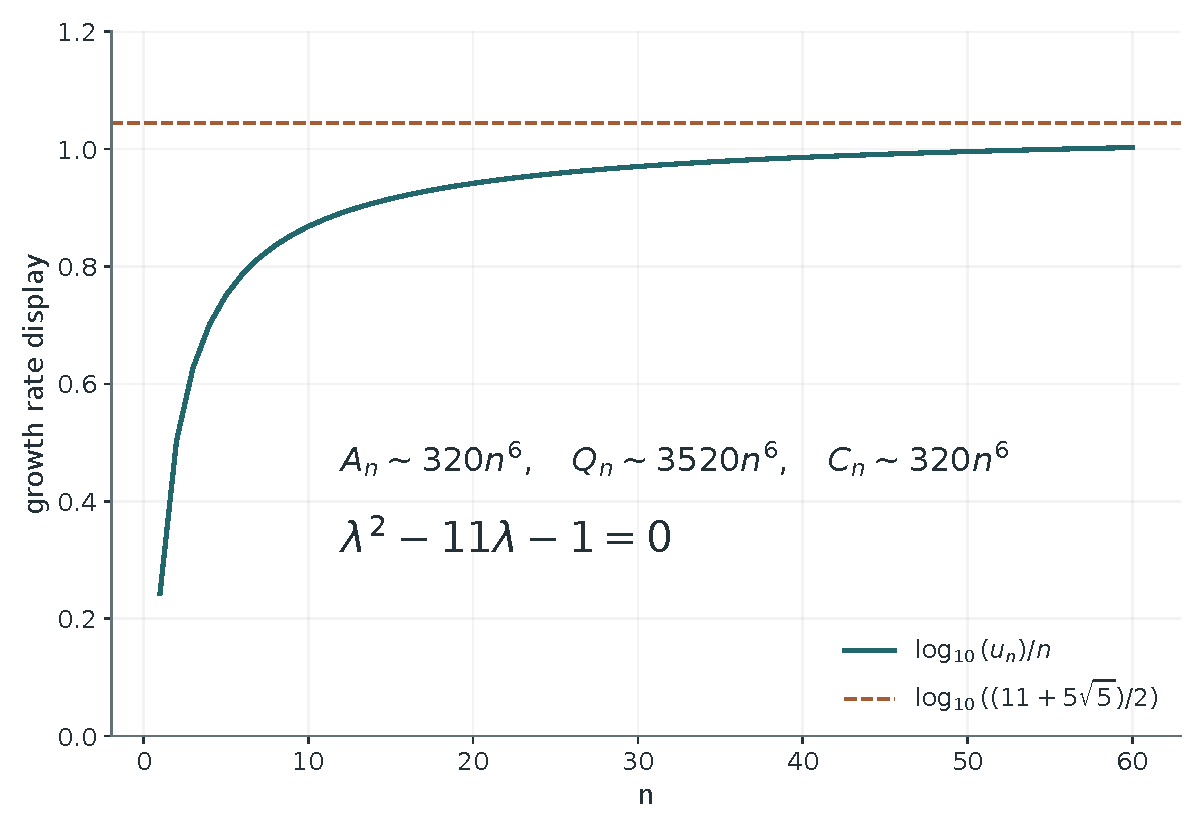
\includegraphics[width=0.92\linewidth]{../visual/figures/11_recurrence_growth.pdf}
\caption{The growing coefficient scale corresponds to the larger
characteristic root. Finite plotted values illustrate the behavior. The
universal limiting rate is a separate source theorem.}
\label{cb_fig_recurrence_growth}
\end{figure}

\section{Normalized error and the arithmetic question}

An immediate consequence of the two source rates is
\begin{equation}\label{cb_eq_ratio_error_rate}
 \lim_{n\to\infty}|G-r_n|^{1/n}
 =\lim_{n\to\infty}\frac{|u_nG-v_n|^{1/n}}{u_n^{1/n}}
 =\phi^{-10}.
\end{equation}
Thus the ratio error has a smaller exponential scale than the unnormalized
linear form. The distinction comes from division by the growing
coefficient $u_n$. Also, since $r_n\to G>0$, one has
$r_n^{1/n}\to1$ and consequently $v_n^{1/n}\to\phi^5$. Both individual
sequences grow, while their specified linear combination decays.

The scaled coefficient used in the packet construction has rate
\[
 \lim_{n\to\infty}(16^nu_n)^{1/n}
 =16\phi^5=88+40\sqrt5.
\]
Chapter~\ref{cb_ch_integrality} proves that this scaled coefficient is an
integer at every index using a separate half binomial identity. Its growth
rate and its integrality are distinct mathematical facts.

\begin{figure}[tbp]
\centering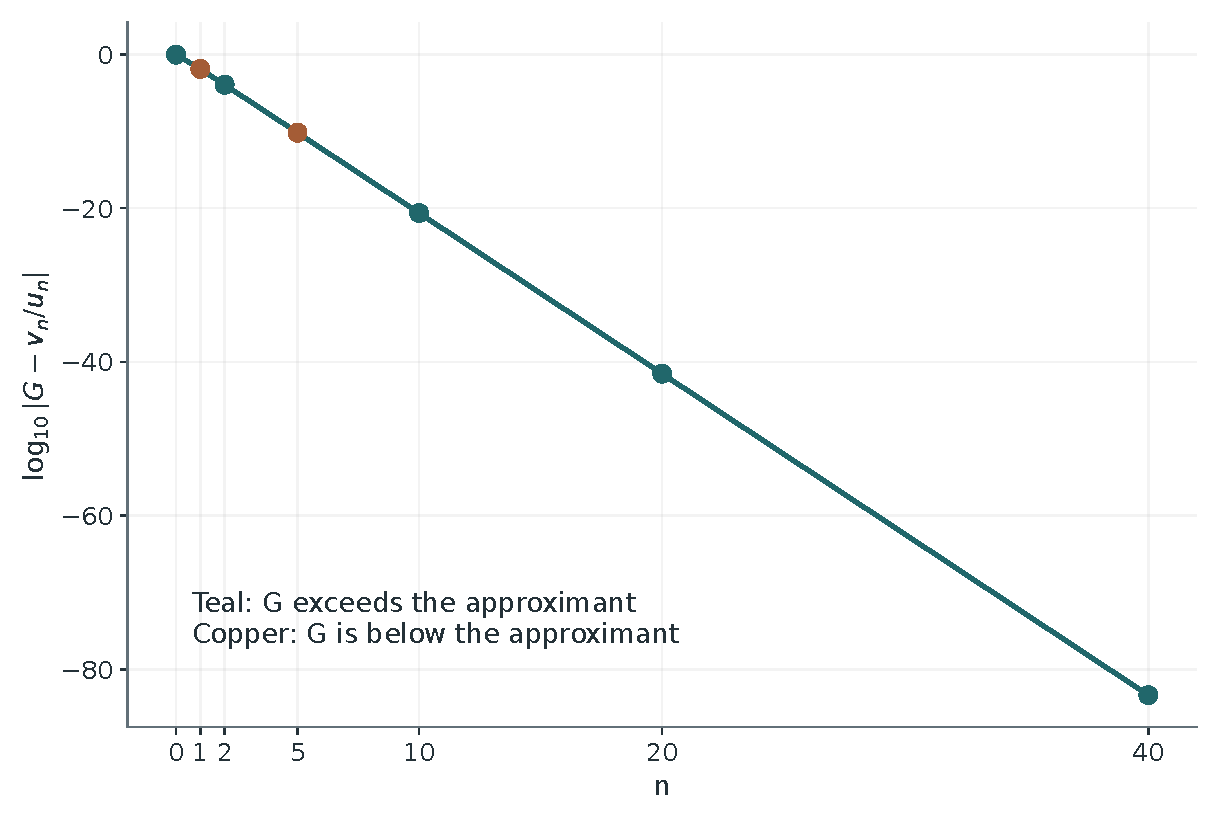
\includegraphics[width=0.92\linewidth]{../visual/figures/12_approximant_error.pdf}
\caption{The normalized rational error decreases rapidly. Exact interval
computations support the finite plotted values. The asymptotic rate
depends on the identified source solution, and irrationality requires
denominator control in addition.}\label{cb_fig_ratio_error}
\end{figure}

The approximants therefore do much more than the original alternating
partial sums in numerical accuracy. Their rapid convergence still does
not classify the limit as irrational. The fractions $u_n$ and $v_n$ carry
denominators, and the denominator of their ratio may grow rapidly too.
To apply the integer lattice criterion, one must turn the error into a
nonzero integer linear form and show that its size tends to zero after
all necessary clearing. The recurrence supplies the coefficients and the
analytic theorem supplies the error scale. The subsequent determinant,
integrality and packet chapters examine the additional arithmetic needed
to connect these facts to that criterion.
